% Backpropagation practice problem (2-3-3-1 network: sigmoid, ReLU, linear; squared error): solution
% for both versions of the handout. Version 1 defines ReLU with slope 0 at x = 0 (Backprop_Practice_Problem.pdf);
% version 2 with slope 1 at x = 0 (Backprop_Practice_Problem-1.pdf). Numbers checked in Python (2026-10-21).
% Build: pdflatex backprop_practice_solution.tex
\documentclass[11pt]{article}
\usepackage[margin=0.85in,top=0.6in,bottom=0.6in]{geometry}
\usepackage[T1]{fontenc}
\usepackage{lmodern}
\usepackage{amsmath,amssymb,bm,tikz,array,xcolor}
\usetikzlibrary{calc}
\usepackage[most]{tcolorbox}
\setlength{\parindent}{0pt}
\setlength{\parskip}{4pt}
\pagestyle{empty}
\definecolor{path}{RGB}{200,90,20}
\newtcolorbox{versionbox}{colback=orange!6,colframe=path,boxrule=0.8pt,arc=2pt,left=6pt,right=6pt,top=2pt,bottom=2pt}

\begin{document}

{\Large\bfseries Backpropagation practice problem: solution}

\begin{center}
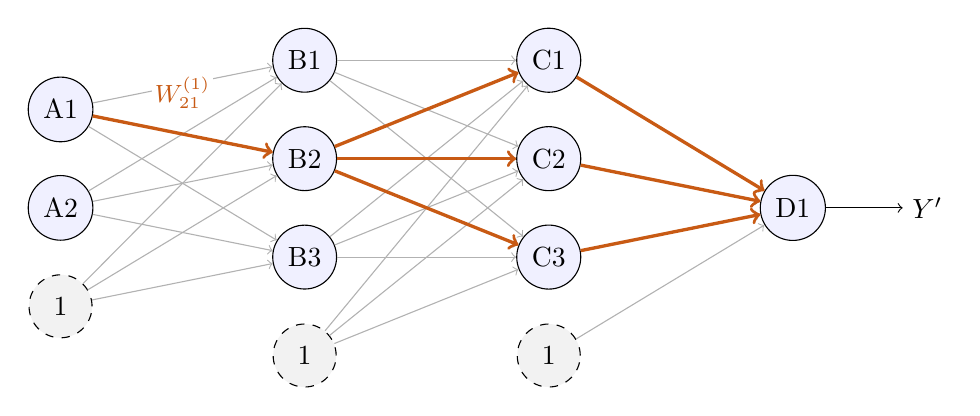
\begin{tikzpicture}[x=3.1cm,y=1.25cm,n/.style={circle,draw,minimum size=8mm,fill=blue!6},
  bn/.style={circle,draw,dashed,minimum size=8mm,fill=gray!10},
  e/.style={->,gray!60}, hp/.style={->,very thick,path}]
\node[n] (A1) at (0,2.5) {A1}; \node[n] (A2) at (0,1.5) {A2}; \node[bn] (A0) at (0,0.5) {1};
\node[n] (B1) at (1,3) {B1}; \node[n] (B2) at (1,2) {B2}; \node[n] (B3) at (1,1) {B3}; \node[bn] (B0) at (1,0) {1};
\node[n] (C1) at (2,3) {C1}; \node[n] (C2) at (2,2) {C2}; \node[n] (C3) at (2,1) {C3}; \node[bn] (C0) at (2,0) {1};
\node[n] (D1) at (3,1.5) {D1};
\foreach \a in {A1,A2,A0} \foreach \b in {B1,B2,B3} \draw[e] (\a) -- (\b);
\foreach \a in {B1,B2,B3,B0} \foreach \b in {C1,C2,C3} \draw[e] (\a) -- (\b);
\foreach \a in {C1,C2,C3,C0} \draw[e] (\a) -- (D1);
% the paths from W^(1)_21 to the loss
\draw[hp] (A1) -- (B2); \node[font=\small,text=path,fill=white,inner sep=1pt] at ($(A1)!0.5!(B2)+(0,0.42)$) {$W^{(1)}_{21}$};
\foreach \c in {C1,C2,C3} {\draw[hp] (B2) -- (\c); \draw[hp] (\c) -- (D1);}
\draw[->] (D1) -- ++(0.45,0) node[right] {$Y'$};
\end{tikzpicture}
\end{center}
{\small The thick lines are the paths along which $W^{(1)}_{21}$, the weight from A1 to B2, affects the
loss: through B2, then through each of C1, C2 and C3, to D1.}

\textbf{Problem.} The B layer uses a sigmoid, the C layer ReLU, and D1 is linear. The loss is squared
error, with $\partial E/\partial Y' = Y' - Y$ (as given in the handout). A record with actual value
$Y = 7$ is passed in. Using the weights and node values below, adjust $W^{(1)}_{21}$ with a learning
rate of 1.

Weights (row $j$ of each matrix holds the weights into node $j$ of that layer):
\[
\bm{W}^{(1)} = \begin{pmatrix} 2.5 & -0.4 \\ 0.2 & 2.6 \\ 1.3 & 1.5 \end{pmatrix},\
\bm{b}^{(1)} = \begin{pmatrix} -1.8 \\ 2.9 \\ 0.7 \end{pmatrix},\quad
\bm{W}^{(2)} = \begin{pmatrix} -1.2 & 0.7 & 2.7 \\ 0.3 & 0.5 & -0.4 \\ 1.3 & 1.9 & -3.4 \end{pmatrix},\
\bm{b}^{(2)} = \begin{pmatrix} 0.9 \\ 1.2 \\ 2.2 \end{pmatrix},
\]
\[
\bm{W}^{(3)} = \begin{pmatrix} 0.3 & 0.6 & -0.2 \end{pmatrix},\quad b^{(3)} = 0.5 .
\]
Node outputs during the forward propagation (given; no forward pass needed):
\begin{center}
\renewcommand{\arraystretch}{1.15}
\begin{tabular}{|l|l|l|l|}
\hline
A layer & B layer & C layer & D layer \\ \hline
$A_1 = 3$ & $B_1 = -1.5$ & $C_1 = 0$ & $D_1 = Y' = 5.3$ \\
$A_2 = 4$ & $B_2 = 2.5$ & $C_2 = 3.3$ & \\
 & $B_3 = -3.4$ (version 1), $3.4$ (version 2) & $C_3 = 4$ & \\ \hline
\end{tabular}
\end{center}

\textbf{Notation}, as in class: $W^{(l)}_{ji}$ is the weight from node $i$ of layer $l-1$ to node $j$ of
layer $l$ (the handout's $W^l_{ji}$). So $W^{(1)}_{21}$ goes from A1 to B2, and $W^{(2)}_{k2}$ goes from
B2 to C$k$. We write $z$ for a node's input sum (its pre-activation), e.g.\ $z_{B_2}$.

\textbf{The two versions} of the handout differ only in how ReLU treats an input of exactly 0:

\begin{center}
\renewcommand{\arraystretch}{1.15}
\begin{tabular}{|l|l|l|}
\hline
& \textbf{ReLU} & \textbf{ReLU slope} \\ \hline
Version 1 & $f(x) = 0$ if $x \le 0$; \ $f(x) = x$ if $x > 0$ & 0 if $x \le 0$; \ 1 if $x > 0$ \\ \hline
Version 2 & $f(x) = 0$ if $x < 0$; \ $f(x) = x$ if $x \ge 0$ & 0 if $x < 0$; \ 1 if $x \ge 0$ \\ \hline
\end{tabular}
\end{center}
(Version 2 also gives $B_3 = 3.4$ instead of $-3.4$, and an $A_3 = 5$ that the network does not have.
Neither $B_3$ nor $A_3$ lies on a path from $W^{(1)}_{21}$ to the loss, so they do not change the answer.)

\newpage
% slightly tighter display spacing so the solution fits on one page
\setlength{\abovedisplayskip}{5pt}\setlength{\belowdisplayskip}{5pt}
\setlength{\abovedisplayshortskip}{3pt}\setlength{\belowdisplayshortskip}{3pt}
\subsection*{Solution}

Work backwards from the loss, one layer at a time.

\textbf{Step 1: the output.} D1 is linear, so its slope is 1 and
\[
\frac{\partial E}{\partial z_{D}} = \frac{\partial E}{\partial Y'} = Y' - Y = 5.3 - 7 = -1.7 .
\]

\textbf{Step 2: the C layer.} Each C$k$ feeds D1 through $W^{(3)}_{1k}$, and then passes the error back
through its ReLU:
\[
\frac{\partial E}{\partial z_{C_k}} = -1.7 \cdot W^{(3)}_{1k} \cdot \operatorname{ReLU}'(z_{C_k}) .
\]
C2 and C3 output positive values (3.3 and 4), so their slope is 1 in both versions:
\[
\frac{\partial E}{\partial z_{C_2}} = -1.7 \cdot 0.6 \cdot 1 = -1.02, \qquad
\frac{\partial E}{\partial z_{C_3}} = -1.7 \cdot (-0.2) \cdot 1 = 0.34 .
\]

\begin{versionbox}
\textbf{This is where the versions differ: C1.} C1 outputs 0, which happens at $z_{C_1} = 0$ or below.
\begin{itemize}\setlength{\itemsep}{0pt}\setlength{\topsep}{2pt}
\item \textbf{Version 1:} an output of 0 means $z_{C_1} \le 0$, where the slope is 0. C1 passes
nothing back:
\[ \frac{\partial E}{\partial z_{C_1}} = -1.7 \cdot 0.3 \cdot 0 = 0 . \]
\item \textbf{Version 2:} here the slope at an input of exactly 0 is 1. We take C1's input sum to
be exactly 0, which is what gives an output of 0 under this definition's $x \ge 0$ branch:
\[ \frac{\partial E}{\partial z_{C_1}} = -1.7 \cdot 0.3 \cdot 1 = -0.51 . \]
(If $z_{C_1}$ were negative instead, the slope would be 0 and the answer would be the same as in
version 1.)
\end{itemize}
\end{versionbox}

\textbf{Step 3: B2 adds up the three paths.} B2 feeds C1, C2 and C3 through $W^{(2)}_{12} = 0.7$,
$W^{(2)}_{22} = 0.5$ and $W^{(2)}_{32} = 1.9$, so
\[
\frac{\partial E}{\partial B_2} = \sum_k \frac{\partial E}{\partial z_{C_k}}\, W^{(2)}_{k2}
= \frac{\partial E}{\partial z_{C_1}} \cdot 0.7 + (-1.02) \cdot 0.5 + 0.34 \cdot 1.9 .
\]
\[
\text{Version 1:} \quad 0 - 0.51 + 0.646 = 0.136 . \qquad
\text{Version 2:} \quad -0.357 - 0.51 + 0.646 = -0.221 .
\]

\textbf{Step 4: through B2's sigmoid.} The sigmoid's slope is $B_2(1 - B_2) = 2.5 \cdot (1 - 2.5) = -3.75$,$^{*}$ so
\[
\frac{\partial E}{\partial z_{B_2}} = \frac{\partial E}{\partial B_2} \cdot (-3.75) .
\]
\[
\text{Version 1:} \quad 0.136 \cdot (-3.75) = -0.51 . \qquad
\text{Version 2:} \quad -0.221 \cdot (-3.75) = 0.8288 .
\]

\textbf{Step 5: the weight.} $z_{B_2} = W^{(1)}_{21} A_1 + W^{(1)}_{22} A_2 + b^{(1)}_2$, so
$\partial z_{B_2} / \partial W^{(1)}_{21} = A_1 = 3$:
\[
\frac{\partial E}{\partial W^{(1)}_{21}} = \frac{\partial E}{\partial z_{B_2}} \cdot A_1:
\qquad \text{Version 1: } -0.51 \cdot 3 = -1.53, \qquad
\text{Version 2: } 0.8288 \cdot 3 = 2.4863 .
\]

\textbf{Step 6: the update}, $W \leftarrow W - \eta\, \partial E/\partial W$ with $\eta = 1$:
\[
\text{Version 1: } W^{(1)}_{21} \leftarrow 0.2 - (-1.53) = \mathbf{1.73}, \qquad
\text{Version 2: } W^{(1)}_{21} \leftarrow 0.2 - 2.4863 = \mathbf{-2.2863} .
\]

One node's slope, at C1, changes the sign of the update: in version 1 the path through C1 is switched
off, and in version 2 it carries enough error to outweigh the other two paths.


{\footnotesize $^{*}$The node values were made up for practice. A real sigmoid always outputs a value between 0
and 1, so its slope $B(1 - B)$ is always positive.}
\end{document}
